\documentclass[10pt]{article}
\usepackage{a4wide,epsfig}

\def\alonzo{{A$\lambda$onzo}}


\addtolength{\textheight}{1.5cm}
\addtolength{\textwidth}{1cm}

\pagestyle{empty}

\begin{document}
%\subsection*{\textbf{\LARGE  CURRICULUM VITAE}}
%\begin{center}\textbf{\LARGE  CURRICULUM VITAE} \end{center}

%% \begin{minipage}{15.9cm}
%% \begin{minipage}{10cm}
%% \begin{tabular}{l@{\hspace{1cm}}l}
%% Name:         &          Corina Benzm\"uller, b. Mohr \\
%% Address:      &          Schwarzburgstr. 51 \\
%%               &          60318 Frankfurt a. M., Germany \\
%% Nationality:  &          German \\
%% Date of birth:&          06.02.1975  \\
%% \end{tabular}
%% \end{minipage}   
%% \hfill
%% \begin{minipage}{4cm}
%% \vspace*{-.7cm}
%% \phantom{ 
%% 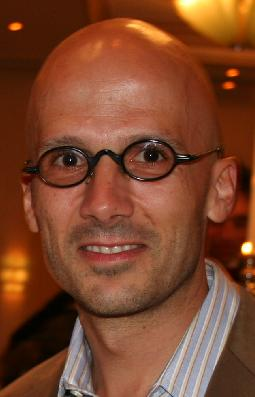
\epsfig{width=3cm,height=4cm,file=chris-2006} 
%% }
%% \end{minipage}
%% \end{minipage}

%% \begin{center}
%% \begin{tabular}{l@{\hspace{.5cm}}l}
%% Name:         &          Corina Benzm\"uller, b. Mohr \\
%% Address:      &          Schwarzburgstr. 51 \\
%%               &          60318 Frankfurt a. M., Germany \\
%% Nationality:  &          German \\
%% Date of birth:&          06.02.1975  \\
%% \end{tabular}
%% \end{center}

\vspace*{-3cm}

\begin{center} \bf
         {\Large PD Dr.-Ing. Christoph E. Benzm\"uller} \\[.5em] %% b. Mohr \\
%         St. Edmunds College, Mount Pleasant, Cambridge Cambridgeshire CB3 0BN, UK \\
%         \& 
% Schwarzburgstr. 51, D-60318 Frankfurt a. M., Germany \\
Saarland University, 66041 Saarbr\"ucken, Germany
%%          German \\
%%          06.02.1975  
\end{center}

\vspace*{.5cm}
\subsection*{\underline{WORK \& RESEARCH EXPERIENCE}}

\noindent
\textbf{Senior Researcher, The University of Cambridge, UK}  \hfill Oct 2006 - Oct 2007 \\
Senior Research Fellow, EPSRC Research Grant: Automation of Higher-Order Logic\\
Visiting Fellow, St. Edmunds College, Cambridge, UK\\[-.5em]

\noindent
\textbf{Associate (\& Assistant) Professor, Saarland University, Germany} \hfill since Jan 2001 \\
Hochschuldozent in Computer Science and co-head of OMEGA research group with 10-15 Researchers\\
Four major research grants in collaborative research center SFB 378 \& several minor grants \\
Scientific head of EU research training network CALCULEMUS (2000-2004)\\[-.5em]

\noindent
\textbf{PostDoc, The University of Birmingham, UK}  \hfill Jan 2000 - Jan 2001 \\
The University of Edinburgh, UK \hfill (3 months)\\
Researcher, EPSRC research grant: Agent-based Theorem Proving \\[-.5em]

\noindent
\textbf{Saarland University, Saarbr\"ucken, Germany}  \hfill May 1995 - Dec 1999 \\
Researcher, DFG research grant: Higher-Order Theorem Proving


\subsection*{\underline{AWARDS}}

%% \textbf{Main Research Grants}\\
%% Agent-oriented Proof Planning, Natural language-based Interaction with a Mathematics Assistance System, Resource-Adaptive Proof Planning, Tutorial Dialogue with a Mathematics Assistance System (all DFG SFB 378 at Saarland University, Germany), Automation of Higher-Order Logic, Agent-based Theorem Proving (both EPSRC, UK), Higher-Order Theorem Proving (DFG) \\

\noindent
\textbf{PostDoc Fellowship, Graduate College Cognitive Science}  \hfill Jan 1999 - Dec 1999\\
Saarland University, Germany\\[-.5em]

\noindent  
\textbf{PhD Scholarship, Studienstiftung des Deutschen Volkes} \hfill Jan 1996 - Dec 1998


\subsection*{\underline{EDUCATION}}
\noindent
\textbf{Saarland University, Saarbr\"ucken, Germany} \hfill since Oct 1989 \\
Habilitation in Computer Science \hfill Jul 2007\\
PhD (Dr.-Ing.) in Computer Science \hfill Jul 1999\\
Diploma in Computer Science with minor subject Economics \hfill Mar 1995\\[-.5em]

\noindent
\textbf{Carnegie Mellon University, Pittsburgh, USA}   \hfill  Jan 1997 - Sep 1997\\[-.5em]

\noindent
\textbf{Gymn. Saarburg/Auguste Victoria Gymn. Trier, Germany} \hfill Aug 1979 - Jul 1988


\subsection*{\underline{ACADEMIC EXPERIENCE}}
\noindent
$>80$ reviewed publications, $>10\times$ chair and $>20\times$ PC member at int.~conferences and workshops, organizer of major scientific events, member of the editorial board of the Journal of Applied Logic, trustee of CALCULEMUS and UITP
communities, $>$ 10 research projects (EU, Germany, and UK), $> 70$ int.~presentations and $>25$ invited talks, $>12$ lecture courses at different universities and summers schools



%% \textbf{Reviewed Publications:} $>$ 80 (in books, journals, conferences \& workshops)\\
%% \textbf{Conferences \& Workshops:} 10 x chair, 15 x programme committee member   \\
%% \textbf{Organization:} CALCULEMUS EU midterm review meeting \& int.~summer school\\
%% \textbf{Editorial Boards/Committees:} Journal of Applied Logic, IJCAR steering committee (2004), CALCULEMUS trustee (since 2004), SFB 378, QPQ \\
%% \textbf{Memberships:} Gesellschaft f\"ur Informatik, Deutscher Hochschulverband, Association for Automated Reasoning, American Association for Artifical Intelligence\\
%% \textbf{Project Management/Research Grants:} $>$ 10 research projects (EU, Germany, UK) \\
%% \textbf{Presentations:}  $>$ 70 talks (including 25 invited talks) \\
%% \textbf{Lecture Courses:}  12 at different universities and summer schools \\
%% \textbf{Supervision:} $>$ 8 PhD students $>$ 15 BSc/MSc/Diploma students

\subsection*{\underline{SYSTEMS DEVELOPMENT}}
Higher-Order Theorem Prover LEO-II (Objective CAML, $> 13.000$ lines
of code), Higher-Order Theorem Prover LEO-I (LISP, $> 8.000$ lines of
code), Agent-based Framework OANTS (LISP, $> 9.000$ lines of code),
project co-head: Mathematical Assistance System OMEGA (LISP,
Mozart-Oz, C++, and others, $>100.000$ lines of code); all systems were
developed under GNU/Linux

\subsection*{\underline{OTHERS}}
\noindent
\textbf{Language Skills:} German (mother tongue), English (fluent), Luxemburgian\\
\noindent
\textbf{Hobbies:} Running (former German champion), scuba diving, skiing, trekking, traveling

\vspace*{1cm}

\begin{flushright}{\bf PD Dr.-Ing. Christoph E. Benzm\"uller\\ December 2007, Frankfurt am Main}
\end{flushright}
\end{document}

%%% Local Variables: 
%%% mode: latex
%%% TeX-master: "cv-short-2007"
%%% End: 
